\chapter{Struttura del controllore}
\graphicspath{{media/1_intro}}
Per il sistema di controllo si è optato per un controllore decentralizzato che comandasse i singoli giunti in maniera indipendente.

La simulazione è stata ottenuta con i tools SImulink e Simscape di MATLAB.

Per ogni giunto si è scelto di implementare un controllore PID in configurazione cascade control. L'anello di controllo più interno controlla la velocità del manipolatore e presenta un guadagno proporzionale molto elevato, mentre l'azione integrale e derivativa sono spente per garantire la stabilità del controllore. L'anello più esterno controlla la posizione ed è stato implementato un controllore PI. 

% schema cascade control
\vspace{20pt}
\begin{tikzpicture}[%
	thick,
	>=latex',
	block/.style={draw, rectangle, minimum width=1.5cm, minimum height=1.2cm, align=center},
	sum/.style={draw, circle, inner sep=1.5pt, node distance=1cm},
	node distance=2cm
	]
	
	% Nodi principali
	\node (r) at (-1,0) {$x_{ref}(t)$};
	\node[sum] (sum1) at (0.5,0) {};
	\node[block] (Gc1) at (2,0) {$PI$};
	\node[sum] (sum2) at (4,0) {};
	\node[block] (Gc2) at (6,0) {$P$};
	\node[block] (Gp) at (9,0) {$G(s)$};
	\node (y1) at (12,0.5) {$x_{out}(t)$};
	\node (y2) at (11,-0.5) {$\dot{x}_{out}(t)$};
	
	% Linee di segnale principali
	\draw[->] (r) -- (sum1);
	\draw[->] (sum1) -- node[midway, above] {$e_1$} (Gc1);
	\draw[->] (Gc1) -- node[midway, above] {$u_1$} (sum2);
	\draw[->] (sum2) -- node[midway, above] {$e_2$} (Gc2);
	\draw[->] (Gc2) -- node[midway, above] {$u_2$} (Gp);
	
	% --- DUE FRECCE PARALLELE DAL BLOCCO Gp ---
	\draw[->] (Gp.east) ++(0,0.25) -- ++(1,0) |- (y1.west);
	\draw[->] (Gp.east) ++(0,-0.25) -- ++(0.25,0) |- (y2.west);
	
	% Feedback interno (secondario)
	\draw[->] (y2.south)|- ++(0,-0.5) -| (sum2.south);
	
	% Feedback esterno (primario)
	\draw[->] (y1.south) |- ++(0,-2.5) -| (sum1.south);
	
\end{tikzpicture} \vspace{20pt}

Si è scelto di fornire nella simulazione direttamente le posizioni calcolate ai giunti della traiettoria, invece che fornire la traiettoria nello spazio di lavoro e determinare nell'ambiente Simscape tramite function block la cinematica inversa, poiché già precedentemente determinate nella simulazione.

\begin{figure}[tbph!]
	\centering
	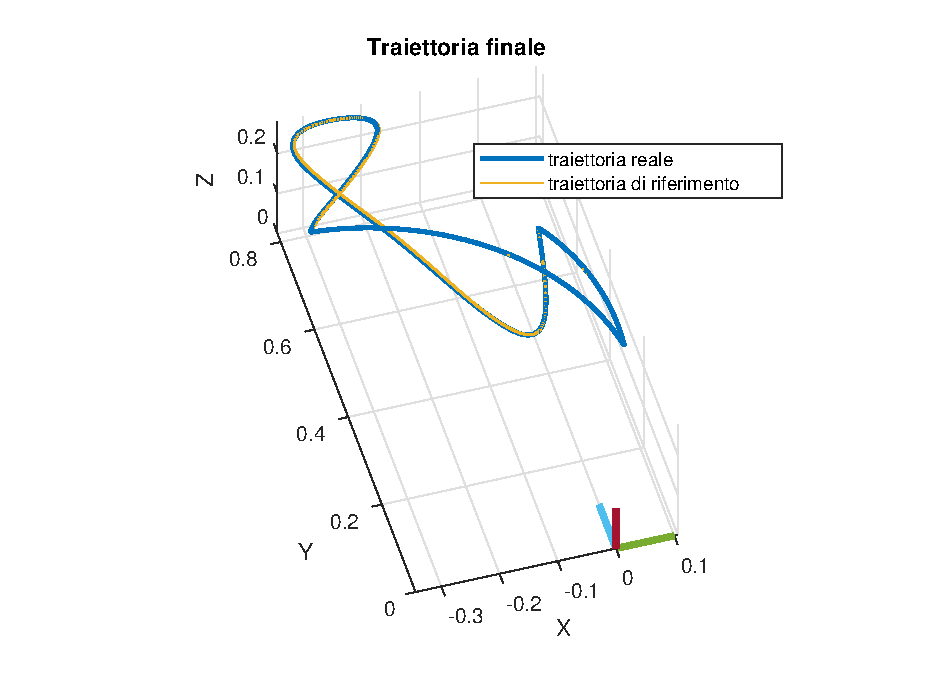
\includegraphics[width=1\linewidth]{media/4_control/traiettoria_finale}
	\caption{Confronto tra la traiettoria di riferimento e la traiettoria compiuta dal robot.}
	\label{fig:traiettoriafinale}
\end{figure}
